\begin{figure}
	\centering
	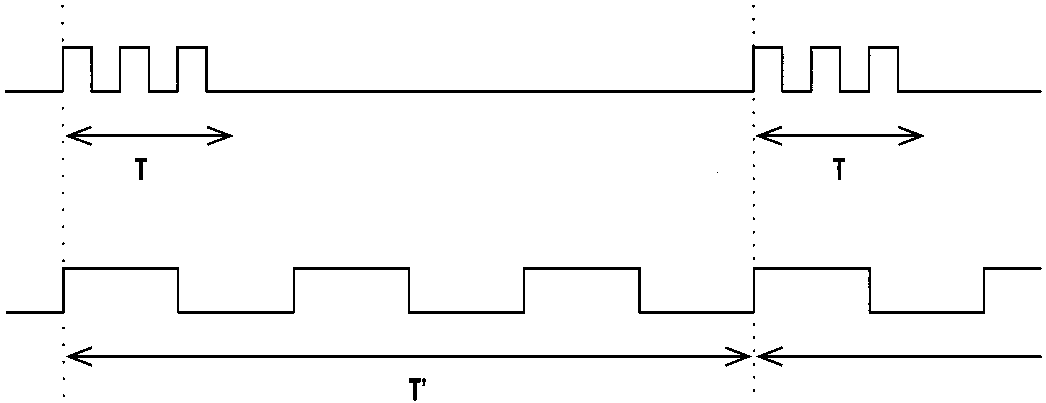
\includegraphics[width=\columnwidth]{../../images/burstycomputation.png}
	\caption{Bursty computation and its relevance to subthreshold operation \cite{IEEEVLSIRobustSTL}}
	\label{fig:burstST}
\end{figure}

\begin{columns}
	\begin{column}{0.5\textwidth}
		\begin{figure}
			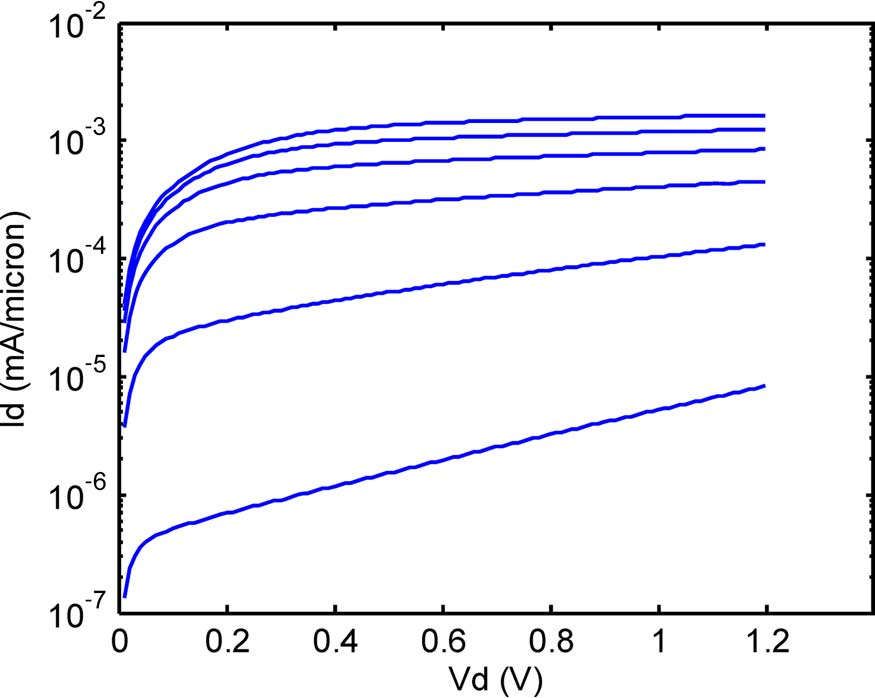
\includegraphics[width=350px]{../../images/vgsvsids.png}
			\caption{$V_{ds}$ vs. $I_{ds}$ \cite{SemiEmpiricalModels}}
			\label{fig:VgsIds}
		\end{figure}
	\end{column}
	\begin{column}{0.5\textwidth}
	\end{column}
\end{columns}

\begin{columns}
	\begin{column}{0.5\textwidth}
	\end{column}
	\begin{column}{0.5\textwidth}
		\begin{figure}
			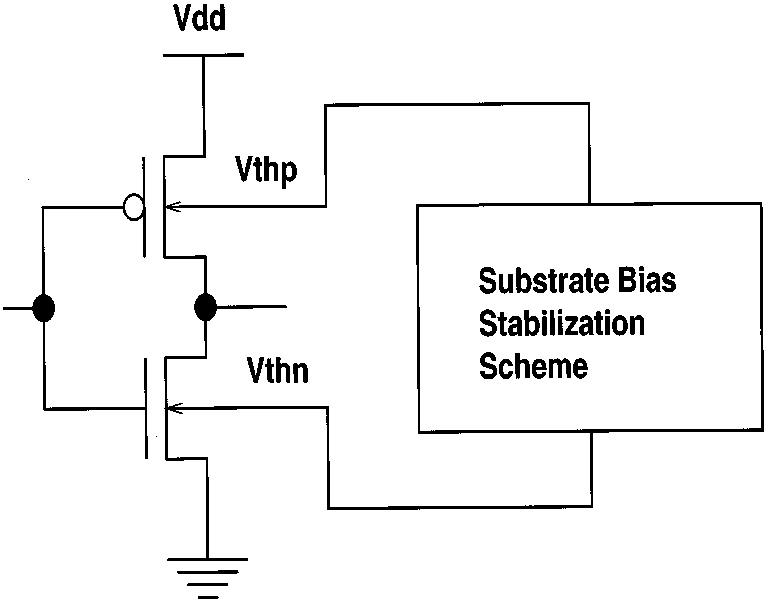
\includegraphics[width=350px]{../../images/vtsubcmos.png}
			\caption{The stabilisation scheme used in VT-Sub-CMOS \cite{IEEEVLSIRobustSTL} }
			\label{fig:vtsubcmos}
		\end{figure}
	\end{column}
\end{columns}
